\subsection{Описание манипулятора}\label{section_description_of_robot}
Основной элемент практически любого робота это~--- манипулятор, в этой работе представленный манипулятором с робота KUKA Youbot и изображённый на рисунке~\ref{img:sizes_of_robot}в. Его механизм имеет пять степеней подвижности. Многозвенная конструкция манипулятора заканчивается двухпальцевым схватом ~--- инструментом, предназначенным для захвата объектов определённой формы.	

Описание технических характеристик дается таблицей~\ref{table_gen_info_of_manipulator} и рисунком~\ref{img:sizes_of_robot}.
%Неуказанные там параметры робота, требуемые для дальнейших расчетов, неизвестны и поэтому подлежат измерению или идентификации, речь о которых пойдет ниже по тексту.

\begin{table}[h!]
	\caption{Общая информация о манипуляторе робота Kuka Youbot.}
	\begin{center}
		\begin{tabularx}{1\textwidth}{|>{\hsize=0.7\textwidth}X|Y|}
			\hline
			\multicolumn{1}{|c|}{Параметр} & \makebox[3cm]{Значение}\\
			\hline
			Количество сочленений & 5\\
			\hline
			Объем рабочей области, $ \text{м}^2 $ & 0.513 \\
			\hline
			Масса, $ \text{кг} $ & 5.3\\
			\hline
			Допустимая нагрузка, $ \text{кг} $ & $0.5$~\\
			\hline
			Точность повторного воспроизведения позиции, $ \text{мм} $ & 1\\
			\hline
			Максимальная скорость в сочленении, $ ^\circ\text{ с}^{-1} $& $90$\\
	    	\hline
			Интерфейс & EtherCAT\\
			\hline
			Напряжение питания, $ \text{В} $ & 24\\
			\hline
		\end{tabularx}
	\end{center}
	\label{table_gen_info_of_manipulator}
\end{table}

\begin{figure}[p]
	\center{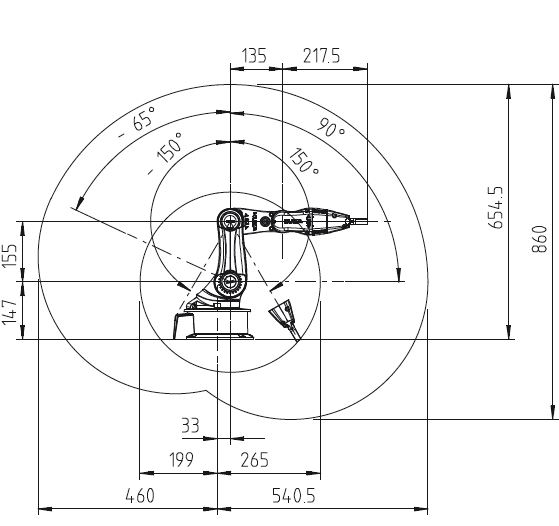
\includegraphics[width=0.7\textwidth]{youbot_workspace_1.jpg} \\ а)}
	\vfill
	\begin{minipage}[h]{0.47\linewidth}
		\centering{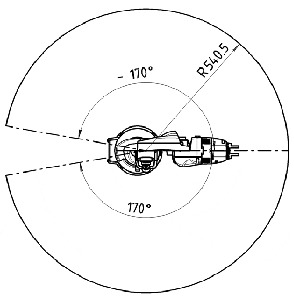
\includegraphics[width=0.95\linewidth]{youbot_workspace_2.jpg} \\ б)}
	\end{minipage}
	\hfill
	\begin{minipage}[h]{0.47\linewidth}
		\centering{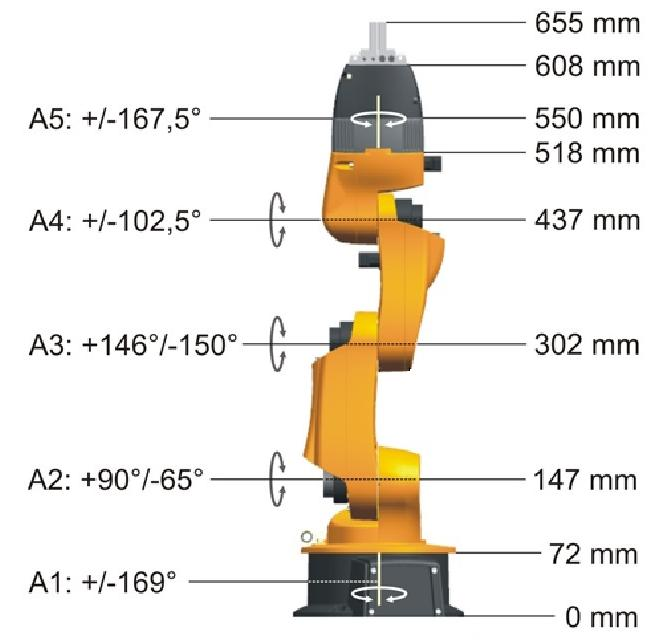
\includegraphics[width=0.95\linewidth]{youbot_length.jpg} \\ в)}
	\end{minipage}
	\caption{Некоторые параметры манипулятора Kuka Youbot: a~--- размеры рабочей области (вид сбоку); б~--- размеры рабочей области (вид сверху); в~--- длины звеньев и предельные значения для углов вращения по каждому из сочленений~\cite{youbot_detailed_specifications}.}
	\label{img:sizes_of_robot}
\end{figure}

%		\hline
%		Поворот 1 сочленения &  $ \pm 169^\circ $\\
%		\hline
%		Поворот 2 сочленения &  $ +90^\circ / -65^\circ$\\
%		\hline
%		Поворот 3 сочленения &  $ +146^\circ / -151^\circ$\\
%		\hline
%		Поворот 4 сочленения &  $\pm 102,5^\circ$\\
%		\hline
%		Поворот 5 сочленения &  $\pm 167,5^\circ$\\
\newpage